



\chapter{Template Chapter}\label{ch:template-chapter}
\section{Images}\label{sec:images}
See Image~\ref{fig:example-picture} on Page~\pageref{fig:example-picture}:
\begin{figure}[hbt!]
    \centering
    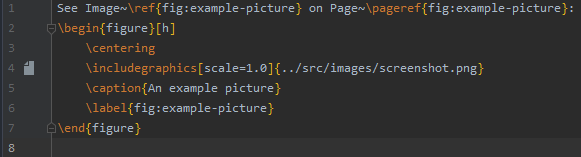
\includegraphics[scale=1.0]{../src/images/screenshot.png}
    \caption{An example picture}
    \label{fig:example-picture}
\end{figure}

Multiple Figures in one environment:
Use hfill for margin between for multi line leave blank lines.
\begin{figure}[hbt!]
    \centering
    \begin{subfigure}[hbt!]{0.49\textwidth}
        \centering
        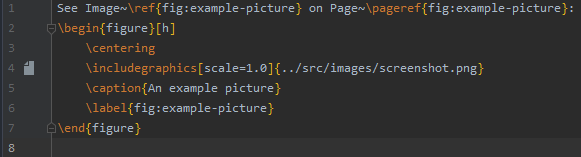
\includegraphics[width=\textwidth]{../src/images/screenshot.png}
        \caption{Picture One}
        \label{fig:one}
    \end{subfigure}
    \hfill
    \begin{subfigure}[hbt!]{0.49\textwidth}
        \centering
        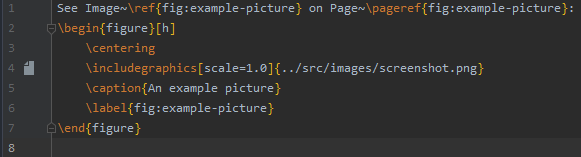
\includegraphics[width=\textwidth]{../src/images/screenshot.png}
        \caption{Picture Two}
        \label{fig:two}
    \end{subfigure}
    \newline
    \begin{subfigure}[hbt!]{\textwidth}
        \centering
        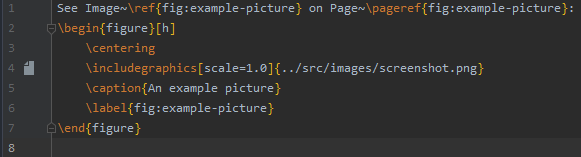
\includegraphics[width=\textwidth]{../src/images/screenshot.png}
        \caption{Picture Three}
        \label{fig:three}
    \end{subfigure}
    \caption{Three pictures}
    \label{fig:three-pictures}
\end{figure}

Reference each fig inside~\ref{fig:three-pictures} like:\newline
One:~\ref{fig:one}\newline
Two:~\ref{fig:two}\newline
Three:~\ref{fig:three}\newline
\clearpage
\section{Tables}\label{sec:tables}
I can reference the table by~\ref{tab:basic-table}
\begin{table}[hbt!]
    \centering
    \begin{tabular}{|l|l|l|}
        A & B & C \\
        \hline
        1 & 2 & 3
    \end{tabular}
    \caption{A basic table}
    \label{tab:basic-table}
\end{table}
See for subtables use:
\begin{table}[hbt!]
    \begin{subtable}[hbt!]{0.45\textwidth}
        \centering
        \begin{tabular}{|l|l|l|}
            A & B & C \\
            \hline
            1 & 2 & 3
        \end{tabular}
        \caption{Multi table 0}
        \label{tab:multi-table-0}
    \end{subtable}
    \hfill
    \begin{subtable}[hbt!]{0.45\textwidth}
        \centering
        \begin{tabular}{|l|l|l|}
            A & B & C \\
            \hline
            1 & 2 & 3
        \end{tabular}
        \caption{Multi table 1}
        \label{tab:multi-table-1}
    \end{subtable}
    \caption{Two tables in one line}
    \label{tab:multi-table}
\end{table}

\section{Minted Code Fragments}\label{sec:minted-code-fragments}

\begin{longlisting}
    \begin{minted}{java}
        public class WaterKettleSteps implements cucumber.api.java8.En {
            @Inject
            public WaterKettleSteps(WaterPage page) {
                When("I waited for \"{int}\" minutes my water is boiling",
                (Integer min) -> {
                    page.assertWaterBoilingAfter(min);
                });
            }
        }

        public class WaterPage {
            public void assertWaterBoilingAfter(Integer min) {
                if (min < 5) { fail(); }
            }
        }
    \end{minted}
    \caption[Short Code Example]{A shorter code example, which will not break across pages.}
    \label{lst:short}
\end{longlisting}

\section{Citation}\label{sec:citation}

Use citation of entry with key rose\textunderscore cucumber\textunderscore 2015: \newline
Citation without brackets with cite\textbraceleft rose\textunderscore cucumber\textunderscore 2015\textbraceright\space like~\cite{rose_cucumber_2015}. \newline
Citation with brackets with parencite\textbraceleft rose\textunderscore cucumber\textunderscore 2015\textbraceright\space like~\parencite{rose_cucumber_2015}.
